% Required packages: pgfplots, lmodern
% Required TikZ libraries: none
% Target width: 160 mm maximum
% Minimum text size: 9 pt
% Colour/greyscale intent: colour_and_greyscale, direct labels and line styles
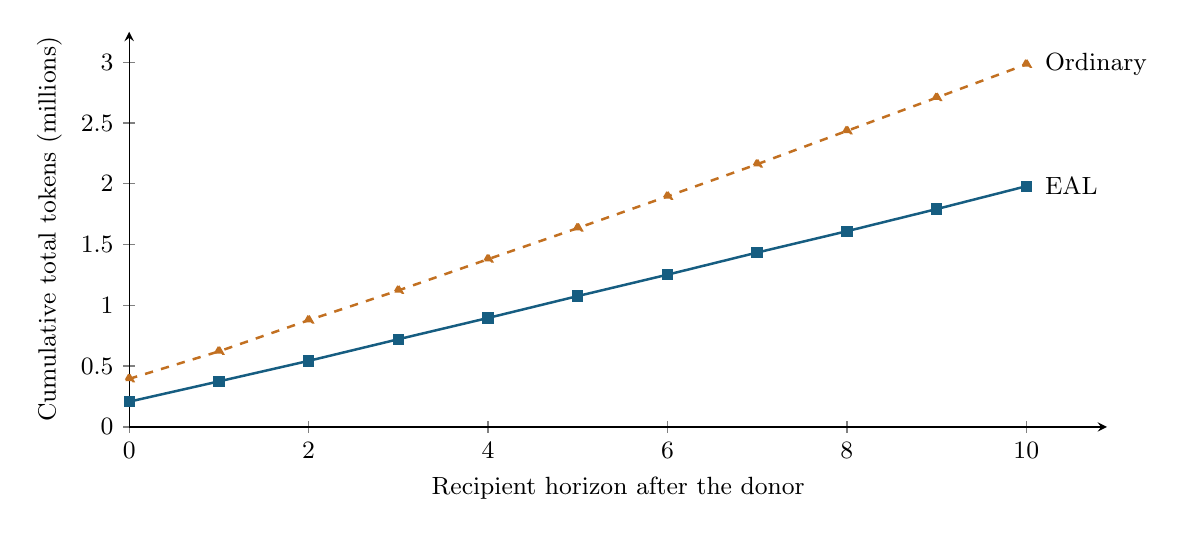
\begin{tikzpicture}
\definecolor{ealblue}{HTML}{165D81}
\definecolor{ordinaryorange}{HTML}{C27021}
\definecolor{neutralgrey}{HTML}{616970}
\pgfplotsset{compat=1.18,
  every axis/.append style={
    width=148mm,height=66mm,
    font=\fontsize{9}{11}\selectfont,
    tick label style={font=\fontsize{9}{11}\selectfont},
    label style={font=\fontsize{9}{11}\selectfont},
    title style={font=\fontsize{10}{12}\selectfont},
    legend style={font=\fontsize{9}{11}\selectfont,draw=none,fill=none},
    axis lines=left,axis line style={line width=0.5pt},
    tick style={line width=0.5pt},
    grid style={line width=0.4pt,black!12},
    scaled ticks=false,clip=false}}
\begin{axis}[width=140mm,height=66mm,xmin=0,xmax=10.9,ymin=0,ymax=3.25,xtick={0,2,4,6,8,10},ytick={0,0.5,1,1.5,2,2.5,3},xlabel={Recipient horizon after the donor},ylabel={Cumulative total tokens (millions)},ymajorgrids=false]
\addplot[ordinaryorange,dashed,line width=0.9pt,mark=triangle*,mark size=1.6pt] coordinates {(0,0.395753) (1,0.621721) (2,0.878065) (3,1.122828) (4,1.37979) (5,1.635867) (6,1.896608) (7,2.160963) (8,2.43503) (9,2.708297) (10,2.982385)};
\node[anchor=west,font=\fontsize{9}{11}\selectfont] at (axis cs:10.1,2.982385) {Ordinary};
\addplot[ealblue,solid,line width=0.9pt,mark=square*,mark size=1.6pt] coordinates {(0,0.207944) (1,0.374917) (2,0.543553) (3,0.721515) (4,0.896522) (5,1.076587) (6,1.252583) (7,1.434602) (8,1.609979) (9,1.792061) (10,1.980029)};
\node[anchor=west,font=\fontsize{9}{11}\selectfont] at (axis cs:10.1,1.980029) {EAL};
\end{axis}
\end{tikzpicture}
